\section*{Dati e risultati}

\subsection*{Amplificatore alle diffrenze}

Lo scopo di questa prima parte è quello di montare un amplificatore alle diffrenze, figura \ref{fig:semplice}, con le seguenti caratteristiche: la corrente di quiescenza $I^q=\SI{0.5}{\milli\ampere}$, un guadagno alle differenze $G\ped{diff} \simeq 30$ e un guadagno in modo comune $G\ped{cm} \simeq 1$.
A tal fine abbiamo posto i seguenti valori per le resistenze: $R\ped{E} = \SI{120}{\ohm}$, $R\ped{C} = \SI{10}{\kilo\ohm}$ che è la resistenza di collettore ed infine $R\ped{1} = \SI{10}{\kilo\ohm}$. Il circuito è alimentato con una tensione di collettore $V\ped{CC}$ di $\SI{15}{\volt}$ e una tensione di emettitore $V\ped{EE}$ di $\SI{-15}{\volt}$.

Il circuito ha 2 entrate, $V_A$ e $V_B$, di cui viene amplifica la differenza ($V_A - V_B$). L'uscita è a singola terminazione.
per verificare il funzionamento del circuito e calcolare il guadagno differenziale, abbiamo alimentato
l'amplificatore con sinusoidi di tensioni picco-picco (tutte le tensioni indicate sono picco-picco) tra $200 \div 400 \; \si{\milli\volt}$
in entrata dal transistor Q1 ($V_A$), mentre il transistor Q2 è posto a terra $V_B = 0$ V.
Uno dei risultati ottenuti è mostrato in figura \ref{fig:f1}.

Per ogni misura abbiamo calcolato il guadagno dividendo l'ampiezza dell'uscita per quella della differenza delle entrate e poi abbiamo mediato i valori ottenuti,
ricavando:

\begin{equation}
    G\ped{diff}\,=\,\frac{V\ped{out}}{V_A-V_B}\,=\, 29.4 \pm 0.3
    \label{eq:G_diff}
\end{equation}

Per ottenere il guadagno in modo comune la procedura è identica con l'unica differenza che abbiamo connesso entrambe le entrate allo stesso segnale sinusoidale.
Un esempio di quello che si ottiene in modo comune è mostrato in figura \ref{fig:f2}.
Si ricava quindi:

\begin{equation}
    G\ped{cm}\,=\,-\frac{V\ped{out}}{V\ped{in}}\,=\, -0.58 \pm 0.01
	\label{eq:G_cm}
\end{equation}
%
dove $V\ped{in}$ indica la tensione picco-picco della sinusoide in ingresso. Si noti inoltre che in questo caso l'uscita è sfasata di 180$^\circ$ rispetto all'entrata,
come si vede dalla figura \ref{fig:f2}.

Infine abbiamo calcolato il CMRR dell'amplificatore seplicemente prendendo il rapporto tra i due guadagni:

\begin{equation}
    \text{CMRR} \,=\,\frac{G\ped{diff}}{G\ped{cm}}\,=\, 51 \pm 1
	\label{eq:cmrr}
\end{equation}


Una volta ottenuto il fattore di reiezione a modo comune possimo stimare la resistenza intrinseca dell'emettitore.
Facendo l'analisi dei piccoli segnali si ottiene:

\begin{equation}
    \text{CMRR} = \frac{R_1}{R_E + r_e} \qquad \implies \qquad r_e = \frac{R_1}{\text{CMRR}} - R_E = 76 \pm 12 \; \Omega
\end{equation}

Infine riportaiamo in figura \ref{fig:f3} uno screenshot dell'oscilloscopio che illustra un caso in cui la tensione in ingresso è troppo alta è
si verifica il clamping.

\begin{figure}
    \begin{subfigure}[t]{0.48\textwidth}
        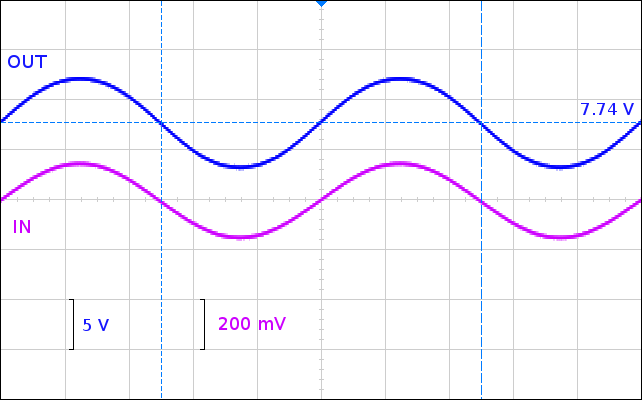
\includegraphics[width=\textwidth]{f1.png}
        \caption{Output dell'amplificatore differenziale con $V_A = 310$ mV (mostrato in figura in viola) e $V_B$ = 0 V.
            Si notino le differenti scale del grafico per i due segnali.
            La tensione picco-picco di uscita è $V\ped{out} = $ 9.2 V. In questa modalità l'uscita è in fase con l'entrata.}
        \label{fig:f1}
    \end{subfigure}
    ~
    \begin{subfigure}[t]{0.48\textwidth}
        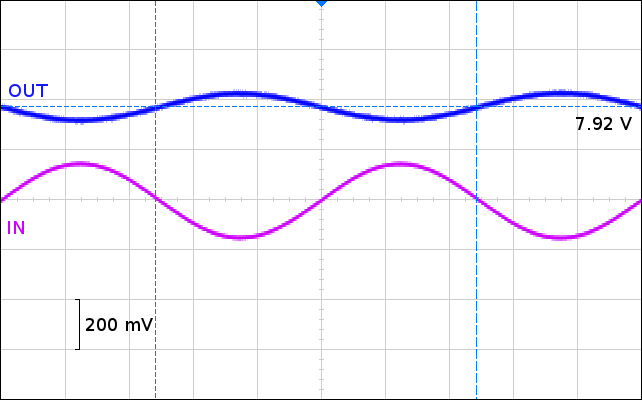
\includegraphics[width=\textwidth]{f2.png}
        \caption{Output dell'amplificatore differenziale con $V_A = V_B$. La tensione picco-picco di ingresso
        è $V\ped{in} =$ \SI{310}{\milli\volt}, mentre in uscita $V\ped{out} = $ -180 mV. In questo caso l'uscita è sfasata di 180$^\circ$ rispetto all'entrata.}
        \label{fig:f2}
    \end{subfigure}
    \begin{subfigure}[t]{0.48\textwidth}
        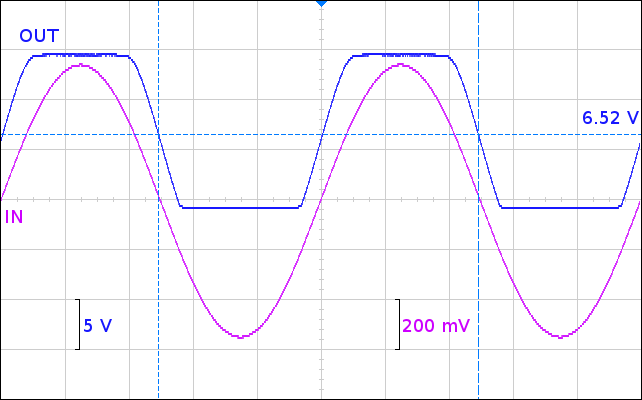
\includegraphics[width=\textwidth]{f3.png}
        \caption{Output dell'amplificatore differenziale con $V_A = 1.1$ V e $V_B = 0$ V. In uscità si ha
        $V\ped{out} = $ 15.4 V. Attensione alla scala dei diversi segnali. Si nota il clamping che l'amplificatore introduce nel segnale.
        Il segnale in uscita non può superare i 15 V dell'alimentazione, come si nota chiaramente, e non può scendere al di sotto a -0.6 V + 0.2 V = -0.4 V (saturazione).
        Infatti sul grafico scende appena sotto lo zero.}
        \label{fig:f3}
    \end{subfigure}
    ~
    \begin{subfigure}[t]{0.48\textwidth}
        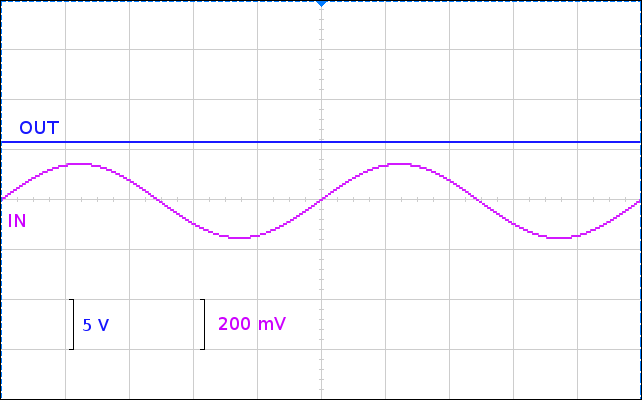
\includegraphics[width=\textwidth]{f4.png}
        \caption{Output dell'amplificatore differenziale migliorato in modo comune. La tensione picco-picco di ingresso
            è $V\ped{in} =$ \SI{300}{\milli\volt}. Si vede il netto miglioramento rispetto al circuito base (figura \ref{fig:f2}), in quanto l'uscita è praticamente costante,
        come ci si aspetta fornendo la stessa tensione a entrambe le entrate.}
        \label{fig:f4}
    \end{subfigure}

    \caption{}
    \label{fig:graphs}
\end{figure}

\subsection*{Amplificatore alle differenze con sorgente di corrente}

In questa seconda sezione vogliamo montare e studiare un amplificatore alle differenze con sorgente di corrente, figura \ref{fig:complesso}.
Questo circuito è un miglioramento del precedente, che, introducendo una sorgente (in realtà un sink) di corrente costante, elimina quasi del tutto
il guadagno in modo comune. Il guadagno in modo comune è evidentemente un difetto, poichè la differenza tra i due segnali è nulla, ma l'amplificatore
da in uscita un segnale non costante. Questo miglioramento permette di aumentare di molto il fattore di qualita (CMRR) dell'amplificatore.

Le caratteristiche di questo circuito sono le seguenti: la resistenza di collettore $R_C$ vale $\SI{10}{\kilo\ohm}$, le due resistenze di emettitore per i transistor Q1 e Q2 hanno lo stesso valore $R_E = \SI{120}{\ohm}$, mentre quelle della sorgente di corrente sono $R_1 = \SI{33}{\kilo\ohm}$, $R_2 = \SI{10}{\kilo\ohm}$ e $R_3 = \SI{1.5}{\kilo\ohm}$.
Il circuito è alimentato a $\SI{+15}{\volt}$ e $\SI{-15}{\volt}$.

Come per il precedente, abbiamo analizzato la risposta del circuito per vari valori di tensione in ingresso, sia in modo differenziale che in modo comune.
Sfruttando le relazioni \eqref{eq:G_diff}, (\ref{eq:G_cm}) e \eqref{eq:cmrr} abbimo ottenuto quanto segue:

\begin{equation}
    G\ped{diff}\,=\, 31.8 \pm 0.4  \qquad\qquad G\ped{cm}\,=\, -0.04 \pm 0.01 \qquad\qquad \text{CMRR}\,=\,\frac{G\ped{diff}}{G\ped{cm}}\,=\, 880 \pm 270
\end{equation}

Come dev'essere il CMRR è molto più grande del precedente.
Per concludere la sezione riportiamo un'immagine, figura \ref{fig:f4}, che mostra l'uscita dell'amplificatore migliorato in modo comune (quella in modo differenziale è uguale
alle figure riportate per il circuito precedente).
